% !TeX root = ../main.tex

\newcommand{\tabincell}[2]{\begin{tabular}{@{}#1@{}}#2\end{tabular}}

\chapter{代码片段相似匹配方法}

本文设计并且实现了基于抽象语法树的相似匹配方法,并且用于第三章的实证研究。由于代码克隆方法首先基于本文对数据的处理结果,本文先介绍了数据的获取步骤和处理步骤;接着,本文介绍提取抽象语法树语法语义特征步骤、以及基于语法特征一致、语义特征使用BLEU(Bilingual Evaluation Understudy)验证相似性的代码克隆匹配步骤。


\section{问题分析与解决思路}
\subsection{问题分析}

\begin{figure*}[htbp]
\centering
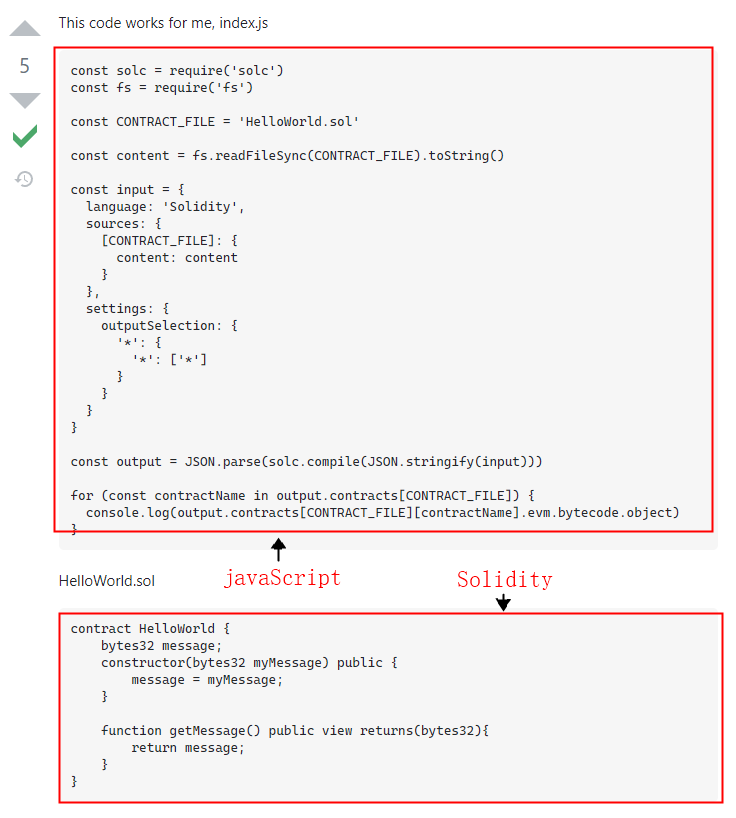
\includegraphics[width=0.6\textwidth]{figures/multi-lan-example.png}
\caption{StackOverflow帖子多语言的例子}
\captionsetup{font={footnotesize}}
\label{multi-lan}
\end{figure*}

代码片段存在于StackOverflow的帖子中,在软件开发过程中,开发者可能学习甚至复制开源社区的代码片段来实现特定的功能。然而,少有人去思考这些代码是否存在漏洞或者存在低效模式。本文的目的是解析问答网站上智能合约有关的漏洞与Gas低效模式分布与两者扩散程度的实证研究。本文经过论文与工具调研,发现以下两个问题。

\begin{itemize}

    \item 代码片段不完整:StackOverflow等问答网站上的代码可能存在多种语言,如\ref{multi-lan}所示,由于Solidity的编译与部署与传统语言不同,它的部署往往依赖Javascript语言。另一方面,不完整的代码片段无法编译。

    \item 如何保证漏洞与Gas低效模式定位一致:相似代码匹配方法用于将开源项目的漏洞与Gas低效模式定位到代码片段,目前没有针对该目的的代码克隆方法。
    
\end{itemize}

\subsection{解决思路}

\begin{figure*}[htbp]
\centering
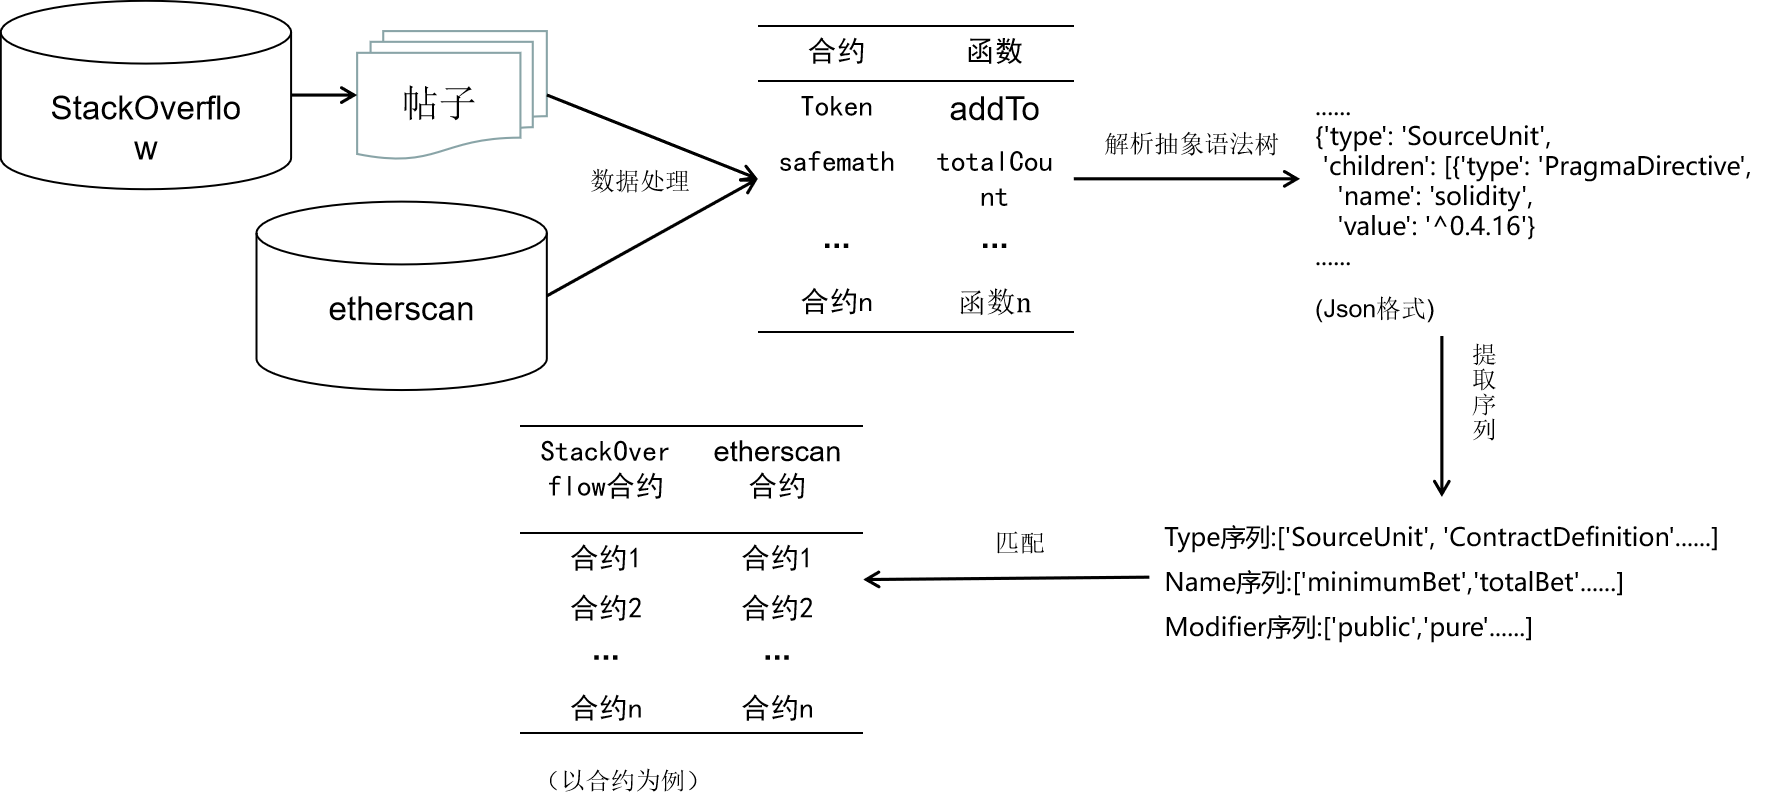
\includegraphics[width=1\textwidth]{figures/chapter2Overview.png}
\caption{代码克隆方法介绍}
\captionsetup{font={footnotesize}}
\label{chapter2Overview}
\end{figure*}

考虑到大部分代码相似度计算方法由于其程序结构不完整,无法用于衡量函数或子类的相似度,为了研究StackOverflow上的不安全与低效代码,并且受限于不同语言下工具的不同,目前在智能合约下尚且没有如Barth等人\cite{partial_java}等人提供的代码片段补全工具。本文将这个任务理解为一个漏洞与Gas低效模式定位的代码克隆问题,即通过代码克隆,找到能够包含代码片段的可编译开源合约,通过对其进行漏洞与Gas低效模式的检测与定位,找到代码片段的漏洞与Gas低效模式;以这种方式,本文能够检测StackOverflow上帖子的安全情况与Gas低效模式分布情况。

代码克隆方法根据它能解决的代码克隆类型作为划分方式。如NICAD\cite{nicad}是一种基于Token的使用优化的最长公共子序列文本比较算法的代码克隆方法,它能够检测类型二代码克隆也就是名称的不一致修改,也能够检测类型三代码克隆也就是由于语句添加或删除产生差异的代码克隆。在它的实现中,根据阈值控制代码克隆相似程度。代码克隆方法的一个使用场景是根据不同需求寻找多个系统的不同程度的代码克隆。

因此本文方法与其他代码克隆检测方法的联系如下所示。

\begin{itemize}
    \item 解析代码:相似代码匹配方法与其他代码克隆方法都通过解析代码进行代码克隆检测,不同的方法与它面向的不同语言使得代码的解析方式不同,有基于文本、基于Token、基于抽象语法树的方法。本文方法基于抽象语法树。
    \item 遵循代码克隆检测类型的逻辑:本文的方法与其他代码克隆方法的检测逻辑一致,根据不同的严格程度,代码克隆的严格程度分为四种,其中类型一最严格即完全相同,类型二其次,一般为名称的不一致,类型三为语句增删改导致的不一致,类型四为语句不一致,功能一致。我们的方法能够检测代码克隆类型一、二与三。
\end{itemize}

我们方法与其他代码克隆检测方法的区别如下所示。

\begin{itemize}
    \item 目的不同:本文的代码克隆方法寻找的是能够保证智能合约上漏洞与Gas低效模式定位一致的代码克隆对,它的代码克检测类型可能跨越类型一、二与三。并且在每种类型中获取其中保证智能合约上漏洞与Gas低效模式定位一致的部分。常见的代码克隆方法更多的寻找如所有类型二或类型三的代码克隆,并不会针对同一类型下的其中的特定代码克隆对。
    \item 场景不同:代码克隆方法的场景常为寻找一个或多个完整代码系统下的不同粒度下的代码克隆,并且将其认为代码异味进行研究。本文的方法将其作为一种StackOverflow下的不可编译代码片段的研究方法;由于不可编译的特点,对代码的解析程度也有所不同,在这里,我们将其解析为常见的中间表示即抽象语法树。
\end{itemize}

同时,本文的相似代码匹配方法与智能合约的相关性如下所示。

\begin{itemize}
    \item 针对智能合约漏洞与Gas低效模式:通过阅读智能合约漏洞与Gas低效模式相关文献,本文发现智能合约漏洞与Gas低效模式与语法信息联系强,而与语义信息联系弱,如Gas低效模式受变量类型,变量定义顺序等语法信息影响大,而受语义信息如变量名、常量值影响小。
    \item 针对StackOverflow下智能合约代码片段无法编译问题:存在使用字节码、程序依赖图进行代码克隆检测的方法,然而代码片段不完整、无法编译的问题使得我们的解析仅能达到抽象语法树的程度。
\end{itemize}

我们的目标是漏洞与Gas低效模式的定位一致。即存在于开源项目的漏洞或Gas低效模式也能够根据代码克隆关系等价的存在于StackOverflow的代码片段上,这与常见的代码克隆方法的检测目标产生区别。我们的代码克隆程度是固定的,也就是能够使得漏洞与Gas低效模式定位一致的代码克隆。目前尚且没有相关的使得漏洞或Gas低效模式定位一致的代码克隆方法。

图\ref{chapter2Overview}展示了第二章方法的整体流程。
接下来,本文介绍了每个步骤的工作。
\begin{itemize}
    \item \textbf{数据处理}:本文收集了来自StackOverflow的代码片段与Etherscan的开源智能合约,并且进行了预处理。由于两种数据粒度不同,本文提取了两种数据的合约与函数用于下一步。
    \item \textbf{解析抽象语法树}:本文的方法是基于抽象语法树的。本文对合约直接使用解析器解析,而对函数额外增加了合约外壳,使其能够正常的解析。
    \item \textbf{提取序列}:本文利用了抽象语法树的三种序列,它们分别是类型序列,名称序列,修饰符序列,本文会将它们转为Hash序列;当两个合约或函数的类型序列与修饰符序列一致时,本文认为达到本文语法一致的目的。
    \item\textbf{匹配}:对于一个来自StackOverflow的合约或者函数,可能有多个来自开源项目库的候选对象与它语法一致。因此本文使用BLEU对候选队列进行匹配,找到BLEU最大的候选项,并且要求BLEU满足阈值,取0.7。
\end{itemize}

%数据格式
\begin{figure*}[htbp]
\centering
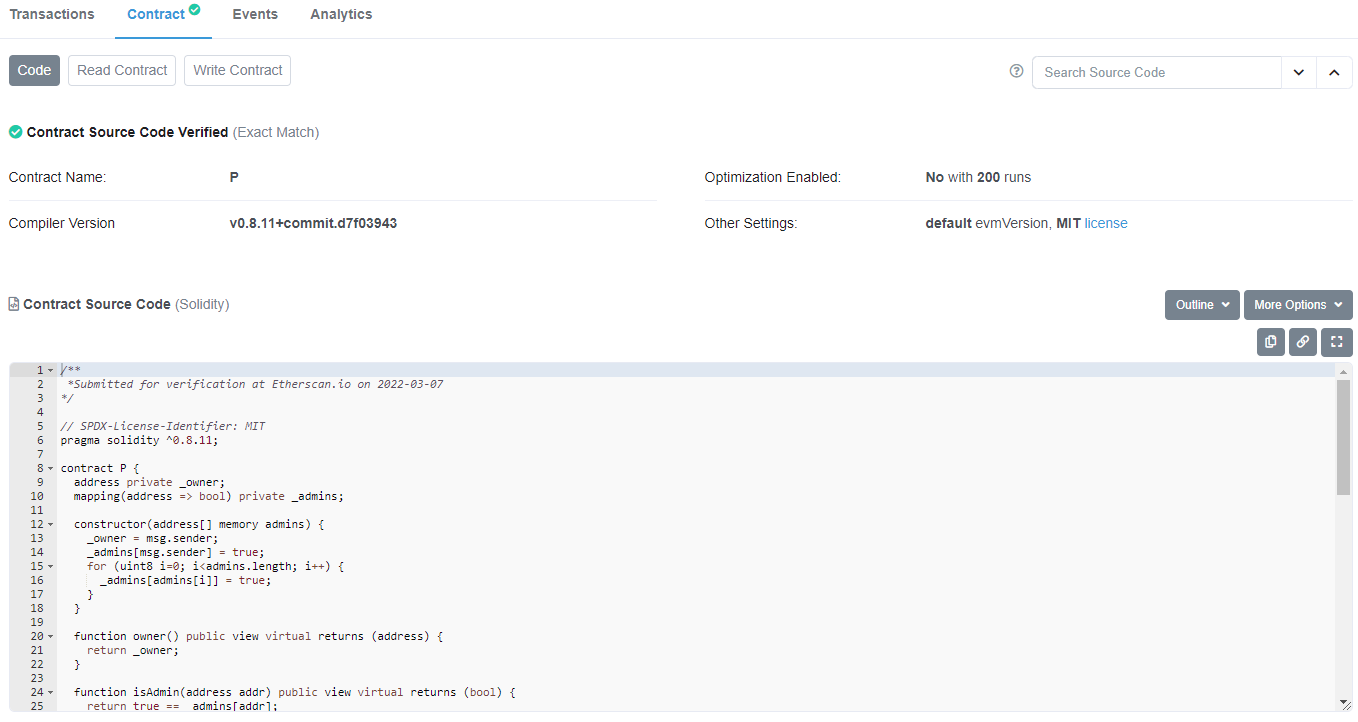
\includegraphics[width=1\textwidth]{figures/etherscan-contract.png}
\caption{Etherscan合约合约界面}
\captionsetup{font={footnotesize}}
\label{etherscan-contract}
\end{figure*}

\section{开源项目与问答网站的数据处理}
本文需要从StackOverflow收集所有与智能合约相关的代码片段,本文首先爬取了2022年1月为止的所有智能合约相关帖子,然后对数据进行预处理。另一方面,本文需要获取开源智能合约,以太坊官网\footnote{\url{https://cn.etherscan.com/}}允许在知道合约地址的情况下下载合约的源代码。因此,本文首先爬取了17万开源项目地址。

对于在以太坊官网获取的开源智能合约项目,它往往以Solidity文件的形式储存。
一个Solidity文件包含多个合约,所谓的合约类似Java或C/C++中类的概念,一个合约可能包含多个函数。

本文使用Python爬虫爬取了从20年6月到21年10月的所有开源智能合约的地址,\ref{etherscan-contract}是Etherscan开源智能合约界面的示例。本文将爬取的数据地址保存到同一个CSV文件,格式如\ref{createFormat}所示,而对单独的开源智能合约项目以Solidity文件形式储存,由于合约地址唯一,因此可以当作主键,本文使用它们的合约地址作为文件名。

\begin{table}[htbp]
\centering
\begin{tabular}{|c|c|c|}
\hline
列名称                         & 类型                  & 注释       \\ \hline
地址                          & string                 & 合约地址     \\ \hline
创建时间                        & datetime & 合约创建时间   \\ \hline
区块号                         & int                  & 合约被打包区块号 \\ \hline
创建交易号 & int                & 合约创建时交易号 \\ \hline
创建者   & int                  & 创建者id    \\ \hline
\end{tabular}
\caption{开源项目数据存储格式}
\label{createFormat}
\end{table}



由于智能合约的复杂部署过程,StackOverflow 中的很多问题都包含与部署相关的 JavaScript 或者 shell 指令。在很多情况下,并不是 StackOverflow 中的所有 Solidity 代码都会直接运行,它们可能会以部分代码片段的形式出现,例如一个函数,或者几行代码。

% %数据格式
% \begin{figure*}[htbp]
% \centering
% 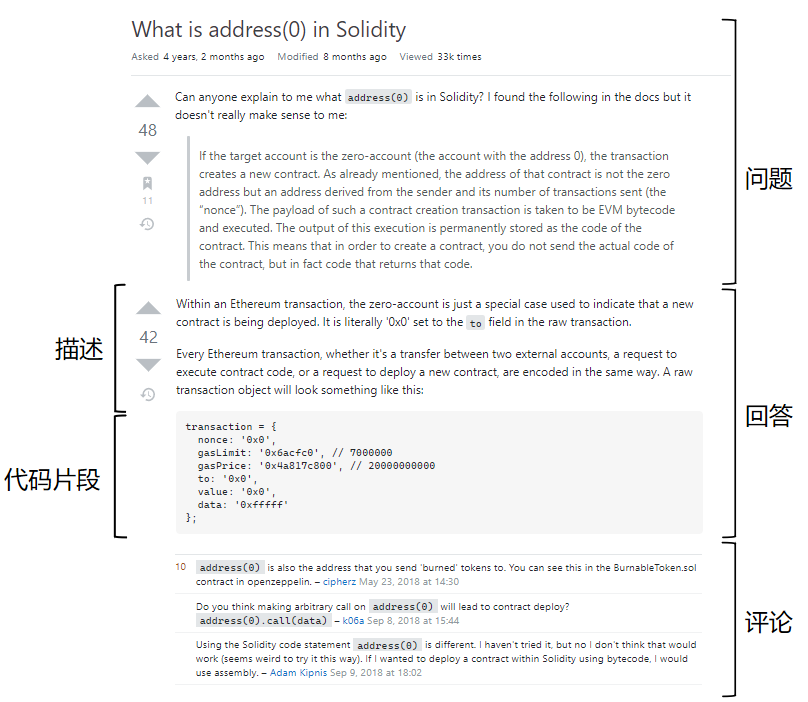
\includegraphics[width=0.7\textwidth]{figures/StackOverflow-example.png}
% \caption{StackOverflow帖子界面}
% \captionsetup{font={footnotesize}}
% \label{so-post}
% \end{figure*}
%,帖子示例如\ref{so-post}
在StackOverflow中,一个帖子有单独的id,帖子下可能有多个答案,答案中可能包含多个代码片段,代码片段通常放在 StackOverflow 帖子中的标签 $<$code$>$页面元素中。本文的存储结构中,先将一个问题或者一个回答视作一个数据,将数据描述储存到同一个CSV文件,具体的代码片段储存为文件。格式如\ref{snippetFormat}。

\begin{table}[htbp]
\centering
\begin{tabular}{|c|c|c|}
\hline
列名称                         & 类型                 & 注释       \\ \hline
Solidity文件名称               & string               & 格式为帖子id-答案数-代码片段数       \\ \hline
提问或回答                     & int                  & 标注代码片段来自提问或者回答   \\ \hline
票数                           & int                  & 对问题或者答案的投票数 \\ \hline
文本描述                       & string               & 对问题或者答案的其余文本 \\ \hline
创建时间                       & datetime             & 创建时间    \\ \hline
\end{tabular}
\caption{StackOverflow代码片段数据存储格式}
\label{snippetFormat}
\end{table}


本文对开源智能合约项目与StackOverflow的代码片段进行以下预处理步骤。

\begin{itemize}

    \item \textbf{去除注释}:对同一份代码文本的注释可能是完全不同的,并且BLEU的输入是有序的词语列表。去除注释是预处理的第一步。在Solidity语言下的注释语法与C/C++的注释语法一致,存在段注释和行注释,对于段注释,本文将删除它所在的整段,对于行注释,本文仅删除行注释标识符及其之后的文本。
    
    \item \textbf{格式规范}:代码编写者之间不会使用统一的编写规范。例如,他们可能在行与行之间键入大量空格。这些格式上的区别对于提取抽象语法树而言是不重要的;统一的代码格式有助于后续的漏洞与Gas低效模式定位步骤。

\end{itemize}

经过上述处理,本文发现代码片段与开源合约项目之间存在很大差异,这是由于不完整的代码片段本质上只是完整项目的一部分。由于本文使用代码克隆方法,因此本文需要对两种代码进行统一处理,得到相同结构的代码。本文的方法是提取两种代码的合约与函数。

当本文爬取的代码片段是无法编译的时候,它仍然保存部分结构信息。本文将它们分类为三种:合约、函数与代码行。这种分类方法基于代码片段是否存在对应结构框体,典型的合约或函数应符合Solidity的语法,并具有固定的合约格式或函数签名;如提取合约时,它会根据Solidity语法,带有“contract”关键字与其对应的语法格式,函数同理;这为本文提取合约或函数提供很大帮助。

本文的工作不对代码行做出处理,这是因为代码行实际上是在一个代码片段中,提取了合约与函数后单独的多段没有结构框体的数据,它们缺少足够的上下文信息,与合约或函数相比,更难确定是否存在漏洞或Gas低效模式。

此外,JavaScript代码在关键字和结构方面与Solidity 代码较为相似,本文现阶段不具体区分这两种代码,而是将它们都提取出来。由于开源项目库中的所有文件都是用Solidity 语言编写的,因此本文可以确保在后续处理可以过滤JavaScript代码,因为JavaScript代码无法匹配Solidity代码。

经过提取处理后的来自开源智能合约项目的合约与函数集合本文称为开源项目库。

\section{基于抽象语法树的克隆对获取}

\begin{algorithm}
\caption{基于抽象语法树的代码克隆检测方法}%算法名字
\label{alg:sim}
\LinesNumbered %要求显示行号
\tcp{$C1$:StackOverflow代码片段}
\tcp{$C2$: 开源项目代码片段}
\tcp{$simScore$:C1与C2的相似分数}

\KwIn{$C1$,$C2$}%输入参数
\KwOut{$simScore$}%输出
% \tcp{当输入为函数时,增加合约框体用于通过智能合约解析器检验}
% \SetKwFunction{FMain}{addContractStructure}
%     \SetKwProg{Fn}{Function}{:}{}
%     %\tcp{如果输入$C$为函数}
%     \Fn{\FMain{$C$}}{
%             \If{isFunction($C$)}{
%                 return $C$ $\gets$ $contractStr$ + $C$
%             }
%             return $C$
%         }
\tcp{计算$C1$与$C2$的相似分数}        
\SetKwFunction{FMain}{getSynSameClone}
    \SetKwProg{Fn}{Function}{:}{}
    \Fn{\FMain{$C1$, $C2$}}{
            \tcp{函数返回结果$simScore$预先置为0}
            $simScore$ $\gets$ 0  \\
            $C1AST$ $\gets$ runAST($C1$)\\ \tcp{运行runAST函数,调用解析器获得抽象语法树} 
            $C2AST$ $\gets$ runAST($C2$) \\
            \tcp{当$C1$或$C2$解析失败时,直接返回}
            \If{$C1AST$ is None or $C2AST$ is None}{
                \Return $simScore$
            }
            \tcp{提取$C1$的语法语义相关序列}
            $C1NameSeries$ $\gets$ getNameSeries($C1AST$) \\
            $C1TypeSeries$ $\gets$ getTypeSeries($C1AST$) \\
            $C1ModifierSeries$ $\gets$ getModifierSeries($C1AST$) \\
            \tcp{提取$C2$的语法语义相关序列}
            $C2NameSeries$ $\gets$ getNameSeries($C2AST$) \\
            $C2TypeSeries$ $\gets$ getTypeSeries($C2AST$) \\
            $C2ModifierSeries$ $\gets$ getModifierSeries($C2AST$) \\
            \tcp{当语法序列一致时计算语义序列的相似度}
            \If{$C1TypeSeries$ = $C2TypeSeries$ and \\ $C1ModifierSeries$ = $C2ModifierSeries$}{
                $simScore$ $\gets$ countBLEU($C1NameSeries$, $C2NameSeries$)
                
            }
            return $simScore$
        }
        
\end{algorithm}

算法\ref{alg:sim}显示了基于抽象语法树的代码克隆检测方法。算法的目的是计算两段合约或者函数的相似程度。

算法的输入是来自StackOverflow的函数或者合约\textit{C1}与来自开源项目的函数或者合约\textit{C2},输出是相似分数\textit{simScore}。

函数\textit{getSynSameClone}接受\textit{C1}与\textit{C2}为输入,首先调用\textit{runAST}函数;\textit{runAST}函数会调用智能合约解析器生成抽象语法树,并以Json格式返回结果,当解析失败时,返回空。\textit{runAST}函数的调用结果分别保存到变量\textit{C1AST}与\textit{C2AST}。当\textit{C1AST}与\textit{C2AST}皆为空时,直接输出\textit{simScore},此时两个代码片段并不相似。

算法提取了三种序列,分别为\textit{NameSeries}序列、\textit{TypeSeries}序列与\textit{ModifierSeries}序列。函数\textit{getNameSeries}、\textit{getTypeSeries}与\textit{getModifierSeries}分别用于遍历以及提取其中的相关节点,以形成序列。

仅当\textit{TypeSeries}序列与\textit{ModifierSeries}序列完全相等时,调用\textit{countBLEU}函数计算\textit{C1NameSeries}序列与\textit{C2NameSeries}序列的相似度。返回相似度结果。

\begin{figure*}[htbp]
\centering
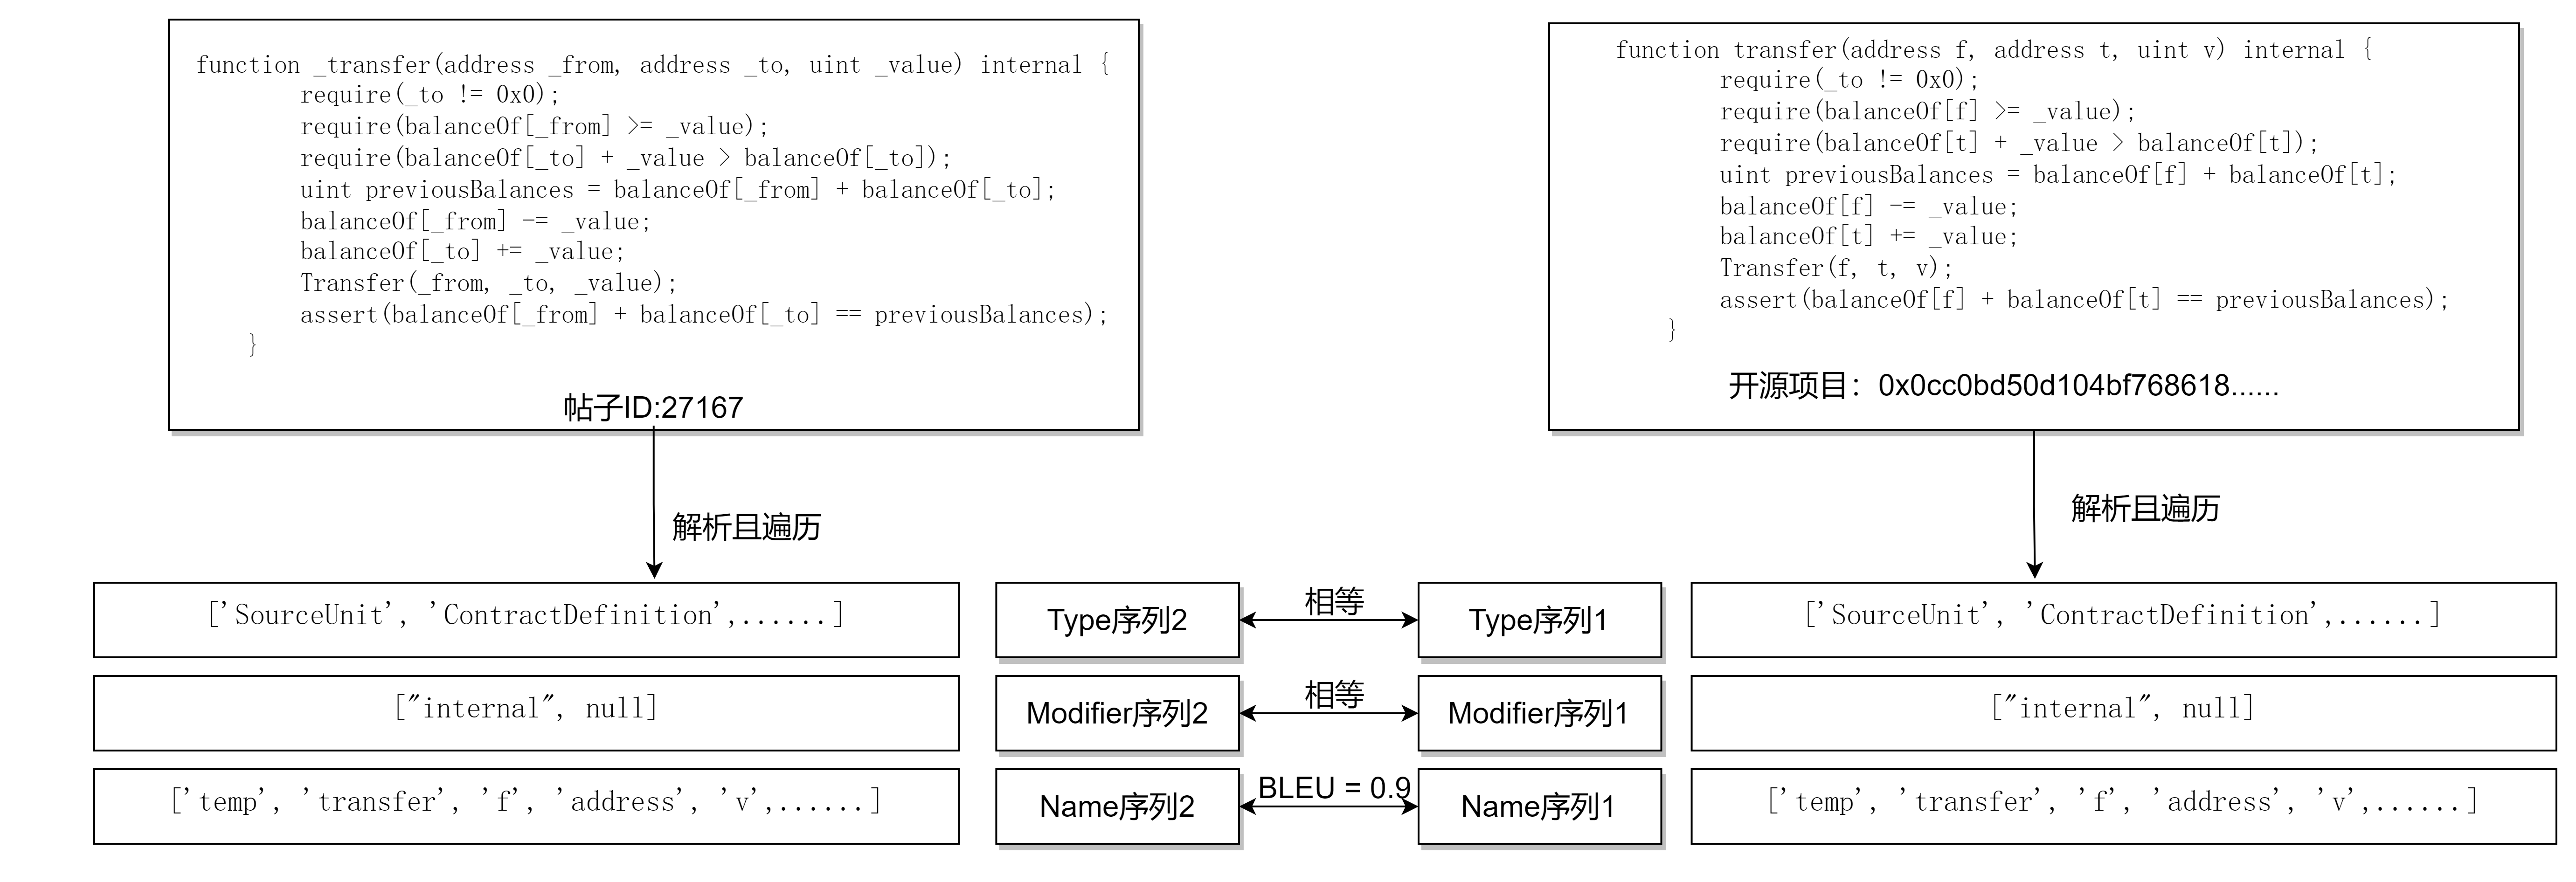
\includegraphics[width=1\textwidth]{figures/methodExample.png}
\caption{算法例子}
\captionsetup{font={footnotesize}}
\label{methodExa}
\end{figure*}

算法例子如\ref{methodExa}所示,对于来自StackOverflow的代码片段与来自开源项目的开源项目中提取的函数,通过解析与遍历步骤,获得三种序列,按照匹配规则后获得相似分数,例子中相似分数为0.9高于设定阈值,因此为相似克隆对。

接下来,本文先介绍抽象语法树的相关概念,如何解析抽象语法树,提取三种Hash序列;寻找相似克隆对需要使用BLEU,本文介绍了BLEU后,介绍基于BLEU的匹配方法,以找到相似的代码克隆对。

\subsection{\label{ast_intro}抽象语法树}

抽象语法树\cite{compilers}是一种用于创建程序的中间表示。编译器通过分析与综合两个步骤将源代码映射为语义上等价的目标程序。分析部分把源代码分解成多个组成要素,并且在要素基础上加上语法结构,然后它使用这个结构创建中间表示。具体来说,经过词法分析、语法分析与语义分析,本文可以得到一个明确的类似机器语言的中间表示。它易于生成并且能够被轻松翻译成目标机器上的语言。

\begin{figure*}[htbp]
\centering

\includegraphics[width=0.3\textwidth]{figures/AST.png}
\caption{编译过程}
\captionsetup{font={footnotesize}}
\label{cpl}
\end{figure*}

\subsubsection{词法分析}

在词法分析步骤,本文对词法分析器输入一个项目的源代码,词法分析器能够将源代码组织成词素(Lexeme)序列,这些词素将对应一个词法单元(Token)。
\[<token\_name, attribute-value> \]

第一个分量token\_name是语法语义分析步骤使用的标识符(identifier),第二个分量attribute-value储存关于这个词法单元的具体信息。
以图\ref{cpl}为例,position是一个词素,被映射成词法单元<id,1>,其中id是标识符(identifier),1指向储存关于这个词法单元的具体信息的位置,存放标识符的相关信息如名字与类型。

\subsubsection{语法语义分析}

抽象语法树时语法分析器通过词法分析器生成的词法单元的Token创建的树形结构。它的每一个内部节点都表示一个运算。

图\ref{cpl}中,“=”节点为根节点,它的左节点是<id,1>节点即position,右节点是“+”节点,“+”节点的子节点信息表明如果要解析“+”节点,必须先算出它的右子节点的结果。同理,运算“=”节点也需要先计算“+”节点。

\subsection{解析抽象语法树}

本文使用了soldity-parser-antlr\footnote{/url{https://github.com/federicobond/solidity-parser-antlr}}的Solidity解析器对两种不同来源的数据进行检测。
它基于antlr\footnote{/url{https://www.antlr.org/}},一种根据语法规则自动生成语法树的开源语法分析器。
抽象语法树生成过程存在静态检查,如合约结构检查。因此在本文的数据中的函数部分,需要额外增加一个合约外壳来通过解析。举例如图\ref{ast-exa},对于一个单独的函数,本文给它合约外壳后,可以通过解析器生成抽象语法树,这个过程中,抽象语法树包含了在编译器中无法被通过的变量a与b,并且保留了语法语义信息。

\begin{figure*}[htbp]
\centering
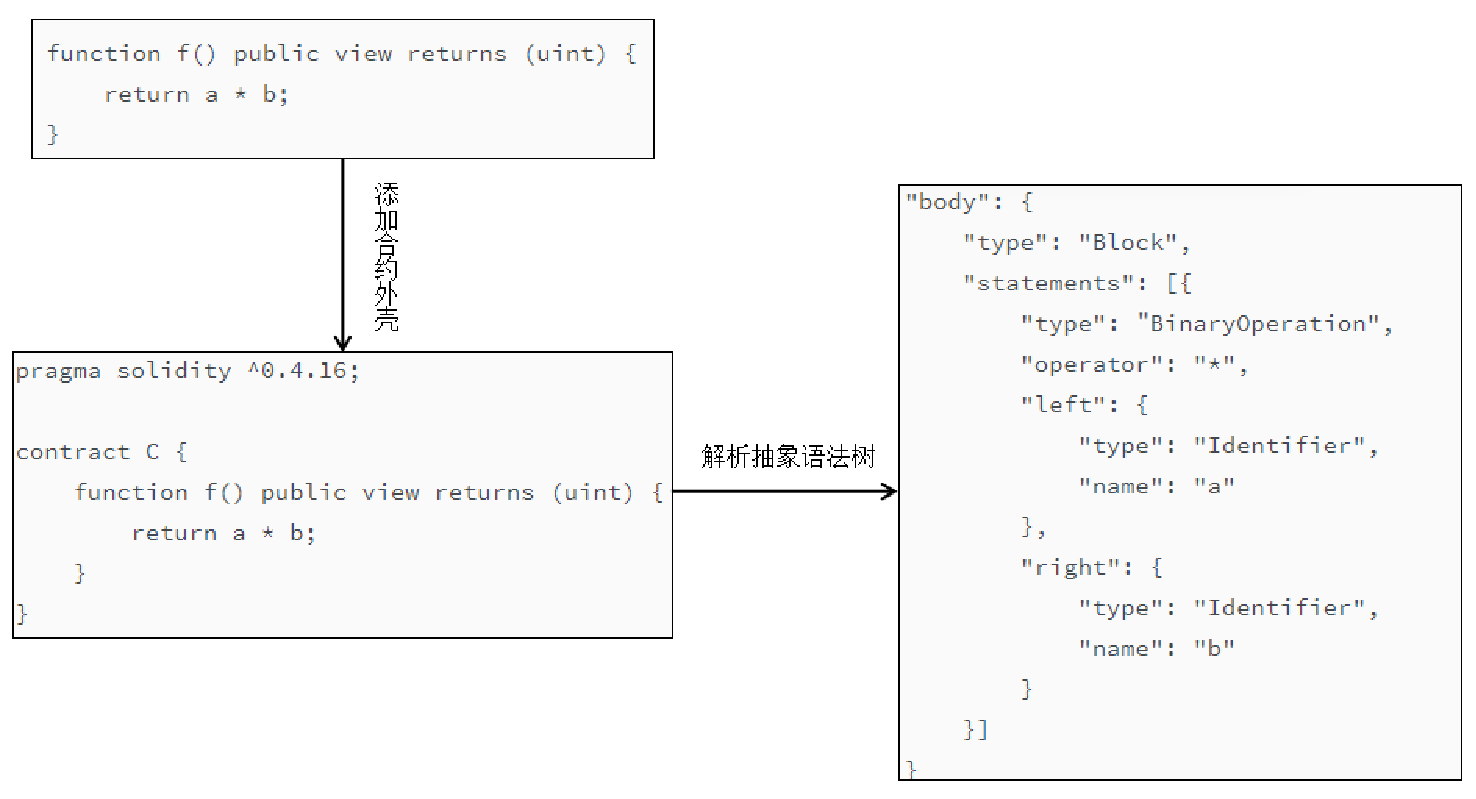
\includegraphics[width=0.8\textwidth]{figures/repair.png}
\caption{抽象语法树编译例子}
\captionsetup{font={footnotesize}}
\label{ast-exa}
\end{figure*}

\subsection{提取序列}

抽象语法树中的每个节点都有一个类型字符串来表示其语法结构的类型。

经验的,通过对漏洞与Gas低效模式相关文献的阅读以及对漏洞与Gas低效模式代码的了解,本文发现从语法语义的角度上,语法信息较大程度的影响漏洞与Gas低效模式的存在,同时语义信息较少的影响。

其中名称为“Type”的子节点标识的它所在子树的数据类型;“Modifier”子节点来自“Type”为“FunctionDefinition”的节点,标识函数的修饰符。更进一步的,“Modifier”子节点包括三种修饰符:“Visibility”、“Modifiers”与“StateMutability”。其中“Visibility”标识函数的公开等级;“Modifiers”标识了函数使用的、由编程人员继承或定义的装饰器。“StateMutability”与Gas相关,不同的取值影响了函数的Gas消耗,具体如下:
\begin{itemize}

    \item \textbf{payable}:附带以太币的调用被payable修饰符修饰的函数时将,以太币将会正常的接收,如果函数不被payable修饰,将会导致调用失败。
    \item \textbf{view}:view修饰的函数只能读取变量值而无法写入。
    \item \textbf{pure}:pure修饰的函数既不能读取变量也不能写入变量。

\end{itemize}

以上对应着代码的语法信息。

对于“Name”序列,它对应的是变量名,函数名,参数名等名称,对应代码的语义信息。

一个抽象语法树可以以树的遍历形式获得序列,本文以前序遍历获得了三种序列。对于包含语法信息的“Type”序列与“Modifiders”序列,本文对节点的值进行Hash获得了Hash序列。本文的算法要求在这两种Hash序列一致的情况下,才能进入到克隆对匹配步骤。对于“Name”序列,本文使用它寻找语义相似而语法一致的克隆对。

使用“Type”序列与“Modifiders”序列是出于本文对漏洞与Gas低效模式的了解,“Type”序列保存了变量类型,语句操作等语法信息;工具根据语法信息使用字节码进行判断,语法一致能够让后续步骤中漏洞与Gas低效模式定位到一致位置。“Modifiders”序列则与某些固定的漏洞或Gas低效模式有关,如Gas低效模式会考虑是否某些函数错误的使用了public关键字导致更高的Gas消耗,同时一些漏洞或Gas低效模式也仅在函数使用public关键字时出现。

\section{基于抽象语法树的克隆对匹配}

\subsection{\label{BLEU}BLEU}

%后续改成使用ccfinder一类根据token的方法
BLEU\cite{bleu}用于自然语言处理中的机器翻译任务,能够评估生成的句子与人工翻译句子的差异程度。为了计算精度,简单的方法在一元精度也就是一个单词的情况下,计算任何参考翻译中出现的候选翻译词的数量,然后除以候选翻译中的总词数。然而,机器翻译系统可能会过度生成“合理”的单词,从而导致不正确但高精度的翻译。直观上,在识别出匹配的候选词后,应将参考词视为已用尽。BLEU将这种直觉形式化为修改后的一元精度。为了计算这一点,首先计算一个单词在任何单个参考翻译中出现的最大次数,称为最大参考计数。接下来,将每个候选词的总计数除以它的最大参考计数,最后计算总和,然后除以候选词的总数。
对于任何n元,修改后的n元精度的计算方式类似:收集所有候选n元精度 计数及其相应的最大参考计数。候选计数被它们相应的参考最大值筛出重复,求和,然后除以候选n元精度的总数\cite{bleu}。

BLEU通常在整个文档的语料库上评估翻译有效性,但基本评估单位是句子。一个源句可以翻译成许多目标句,在这种情况下,首先逐句计算n元匹配,接下来,将所有候选句子的裁剪n元精度 计数相加,然后除以测试语料库中候选n元精度的数量,以计算整个测试语料库的修正精度分数,此时式子如\ref{n-gram}所示。

\begin{equation}
p_{n} = \frac{\sum_{c\in candidates}\sum_{n-gram\in c} Count_{clip}\left ( n-gram\right )}{\sum_{c\in candidates}\sum_{n-gram'\in c'} Count\left ( n-gram'\right )}
\label{n-gram}
\end{equation}

比参考文献长的候选翻译已经受到修改后的n元 精度度量的惩罚,不需要再次惩罚它们。因此,BLEU引入了简洁惩罚因子,此时高分候选翻译必须在长度、单词选择和单词顺序上与参考翻译相匹配。当候选的长度与任何参考翻译的长度相同时。BLEU将最接近的参考句长度称为“最佳匹配长度”,来计算整个语料库的简洁惩罚。BLEU首先通过对语料库中每个候选句子的最佳匹配长度求和来计算测试语料库的有效参考长度。

\subsection{克隆对匹配}

BLEU是一种通过结合一元与多元修改精度,量化机器翻译与其最接近的一个或多个参考人工翻译结果的距离,也就是文本相似问题。当BLEU可以直观的反映文本的相似情况,本文使用BLEU就能够在文本意义上对代码片段进行匹配。

在阅读了基于文本的代码克隆检测方法以及问答网站领域下的相关文献后,本文发现相比于BLEU方法,旧有的基于文本检测方法存在以下问题。

\begin{itemize}
    \item 由于无法利用可编译程序特点,不能针对程序语法语义信息进行检测的基于文本算法优势较小。基于文本的代码克隆检测方法较为久远\cite{Ducasse}\cite{Koschke},并且只能检测完全相同的代码片段。
    \item 代码克隆领域与问答网站领域交互不多,一些存在寻找相似克隆对的情况下,处理较为简单\cite{dicos}\cite{fisher1},在需要确定代码片段相似度的场景下,大多使用Jaccard系数\footnote{{\url{https://en.wikipedia.org/wiki/Jaccard_index}}}。
\end{itemize}

给定两个集合A,B,Jaccard系数定义为A与B交集的大小与A与B并集的大小的比值,定义如\ref{jaccardEquation}:

\begin{equation}
    J\left ( A,B \right ) = \frac{|A\cap B|}{|A\cup B|} = \frac{|A\cap B|}{|A| + |B| - |A\cap B|}
    \label{jaccardEquation}
\end{equation}

Jaccard寻找的是集合A在集合B中的出现频率。并且与BLEU相比,可以发现Jaccard系数与BLEU\cite{bleu}未修改的一元精度方程的定义类似,并且没有考虑到词语顺序与长度不匹配惩罚的问题。
词语顺序或者说语句顺序对于本文的方法是有意义的,比如Gas低效模式中的Sparse storage考虑的就是糟糕的变量定义顺序导致更高的Gas消耗。
因此,本文使用BLEU作为变量名序列匹配的方法。由于过低的BLEU值同样会导致漏洞与Gas低效模式定位不一致,经过手动与经验的检测,本文对其阈值取0.7。

除此之外,BLEU可以作为两个代码段的相似程度的判断指标也在注释生成的相关研究中使用,如Liu等人\cite{bleu-example}将两段代码视作句子,评估代码之间的相似程度;BLEU作为翻译的判断指标,也是一种代码相似程度的判断指标,对于它是否能帮助本文找到相似的代码匹配对,本文在第四章的RQ1中进一步进行实验。

值得注意的是:本文的方法与NICAD类似,通过替换不同的语言解析器即可检测不同语言的代码克隆,对不同语言没有限制,然而不同语言的漏洞不同,因此本方法仅保证了在StackOverflow智能合约代码片段这一场景下的有效性。

\section{本章小结}

本章介绍了基于抽象语法树的代码克隆检测方法。使用StackOverflow的代码片段与来自Etherscan的开源智能合约项目作为数据来源,本文提取了其中的合约与函数作为基本处理单元,并且使用soldity-parser-antlr解析了不同来源的合约与函数,获得了它们的抽象语法树。本文的目标是寻找到语法一致而语义相似的克隆匹配对,处于这个目的,本文对抽象语法树进行前序遍历,提取了三种序列。“Type”序列与“Modifiers”序列保存的语法信息允许本文找到语法一致的匹配对,因此本文对这两种序列进行Hash。“Name”保存了源代码的语义信息,本文使用BLEU作为“Name”序列相似度的计算方法,找到了语法一致情况下,语义相似的代码克隆对。